\documentclass[a4paper]{article}
\usepackage[italian]{babel}
\usepackage[utf8]{inputenc}
\usepackage[T1]{fontenc}
\usepackage{float}
\usepackage{hyperref}
\usepackage{graphicx}
\usepackage{fancyvrb}
\usepackage{fvextra}
\usepackage{csquotes}
\usepackage[backend=biber, style=ieee]{biblatex}
\usepackage{glossaries}
\addbibresource{bibliografia.bib}

\title{Relazione di progetto di Virtualizzazione e integrazione di sistemi\\
\textbf{Server NFS e volumi di container}}
\date{\today}
\author{Luca Casadei\\Matricola: 0001069237}
\makeglossaries

\loadglsentries{defns}
\setacronymstyle{short-long}

\begin{document}
\maketitle

\tableofcontents

\section{Creazione delle macchine virtuali}
In questa sezione verrà indicata la modalità utilizzata per la creazione delle macchine virtuali, 
in particolar modo verrà descritto il modo usato per metterle in comunicazione.
\subsection{Ambiente di virtualizzazione}
Come ambiente di virtualizzazione è stato scelto \textit{Proxmox}, un software debian-based open source che permette di gestire macchine virtuali basato
sull'infrastruttura \gls{KVM} che fornisce già un repository di immagini \gls{LXC}.
\\
Procedo quindi ad un'installazione "fresca" di Proxmox su una workstation, a seguito di tutte le fasi di installazione, mi trovo nella seguente situazione:
\begin{figure}[H]
    \centering
    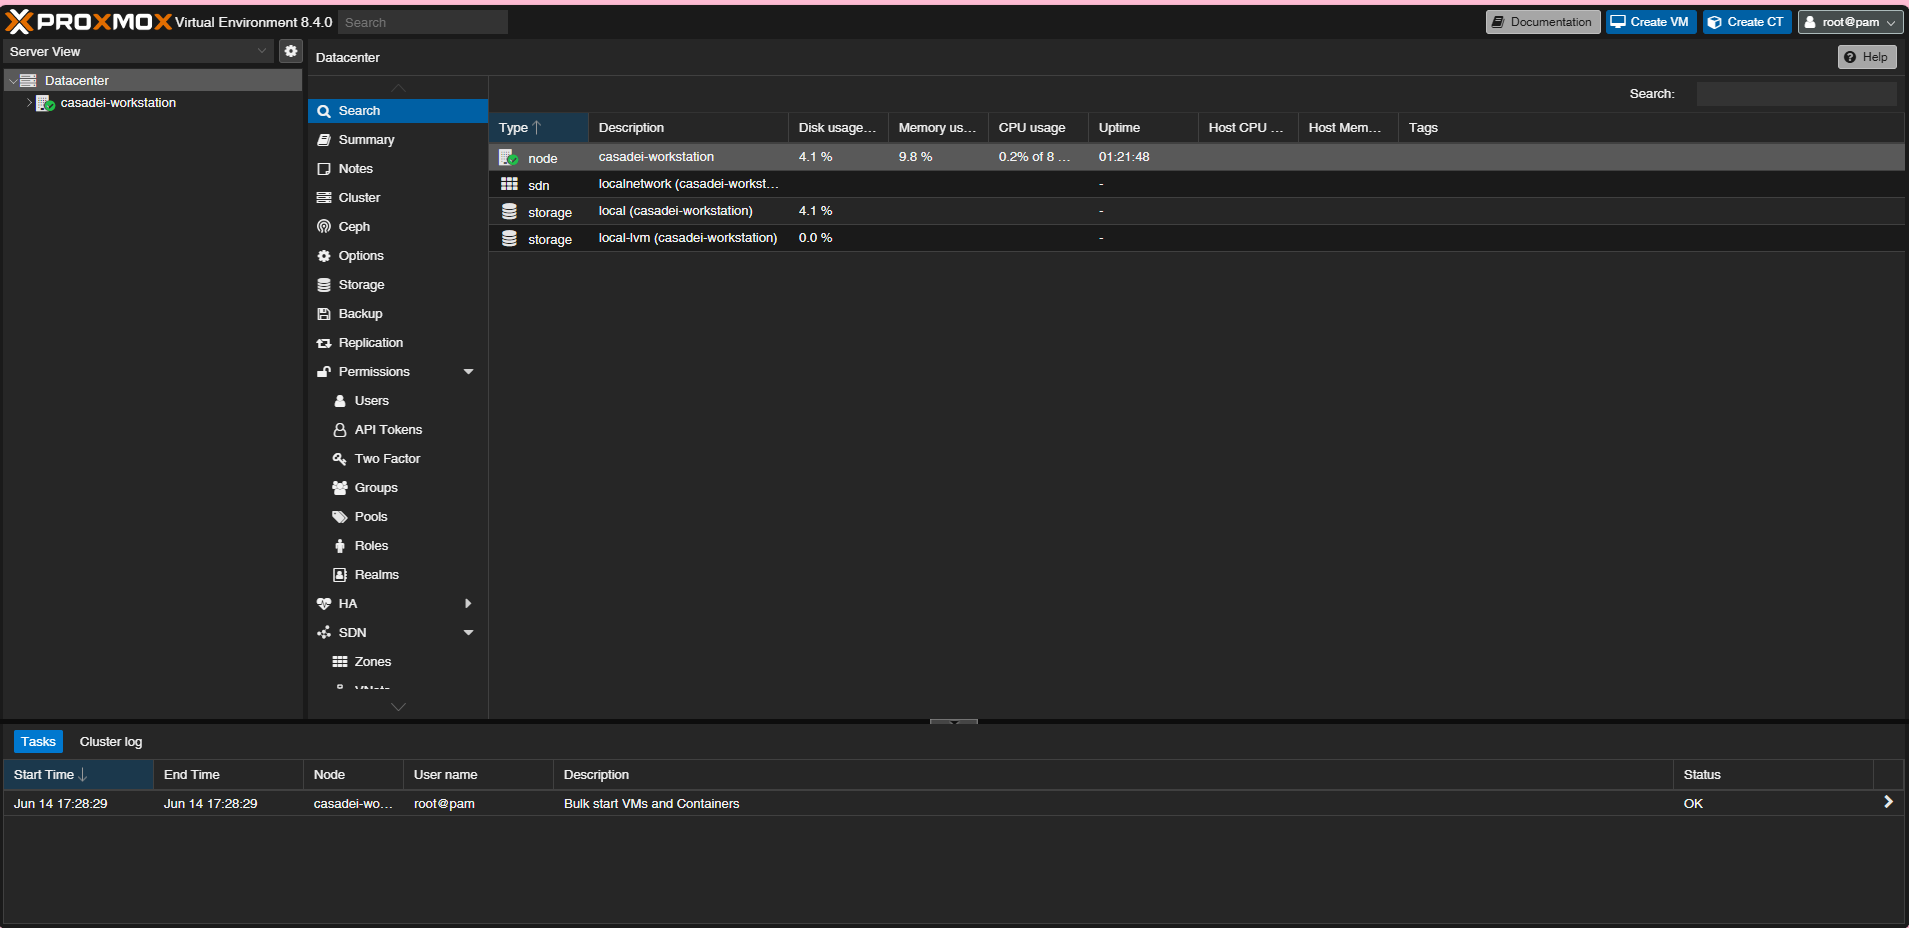
\includegraphics[scale=0.22]{images/ProxMoxDopoInstallazione.png}
    \caption{Proxmox installato su workstation}
\end{figure}

\subsection{Creazione server NFS}
\subsubsection{Cenni su NFS e NFSv4}
Il protocollo \Gls{NFS} versione 4 descritto dalla \cite[rfc7530]{rfc7530} è un'evoluzione dello stesso protocollo in versione 3 e 2 descritti
rispettivamente dalle \cite[rfc1813]{rfc1813} e \cite[rfc1094]{rfc1094}, l'idea alla base del protocollo è quella di rendere accessibile delle
risorse (file) all'interno della rete, indipendentemente dal sistema operativo o architettura di rete. Per realizzare questa astrazione il protocollo
fa uso di primitive chiamate \Gls{RPC} ed una rappresentazione dei dati esterna a quella dei vari sistemi operativi, ma interpretabile da tutti attraverso
la rete, la \Gls{XDR}.\\
NFS era (originariamente) pensato per essere un protocollo stateless, quindi non manteneva informazioni riguardanti i client che ne facevano uso. La versione 2 introduce la possibilità
di gestire file di dimensioni notevolmente superiori rispetto alla versione precedente, oltre all'introduzione di nuove primitive e migliorie a livello di
integrità dei dati in caso di operazioni asincrone.\\
Dalla versione 4, con l'introduzione del file locking (modalità per irrobustire l'integrità dei file trasferiti) il protocollo è necessariamente diventato stateful, rendendo quindi
incompatibili il protocollo in versione 4 e le versioni precedenti, nonostante questo gran parte dei server nfs consentono di configurare il protocollo in più versioni diverse. 

\subsubsection{Effettiva crazione}
Ora andrò a creare la macchina virtuale che conterrà il container per il server NFSv4, non uso un container LXC Proxmox
perché NFSv4 richiede accesso kernel-level. Come sistema da virtualizzare ho scelto Debian 12, che scarico e aggiungo alle ISO
Images di Proxmox (nell'hdd secondario), con il seguente risultato:
\begin{figure}[H]
    \centering
    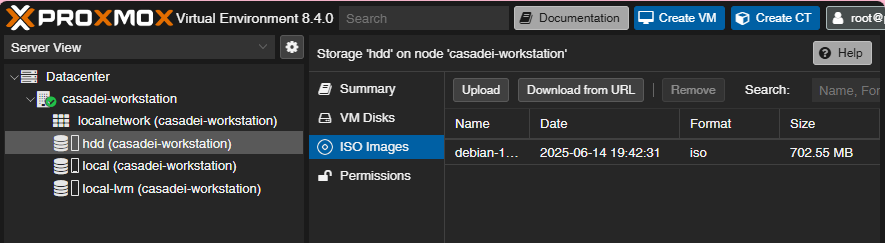
\includegraphics[scale=0.42]{images/IsoDebian12Caricata1.png}
    \caption{Aggiunta ISO Debian 12 a Proxmox}
\end{figure}
Ora procedo a creare la macchina virtuale effettiva seguendo tutte le configurazioni di
Proxmox, questa è la finestra di creazione finalizzata:
\begin{figure}[H]
    \centering
    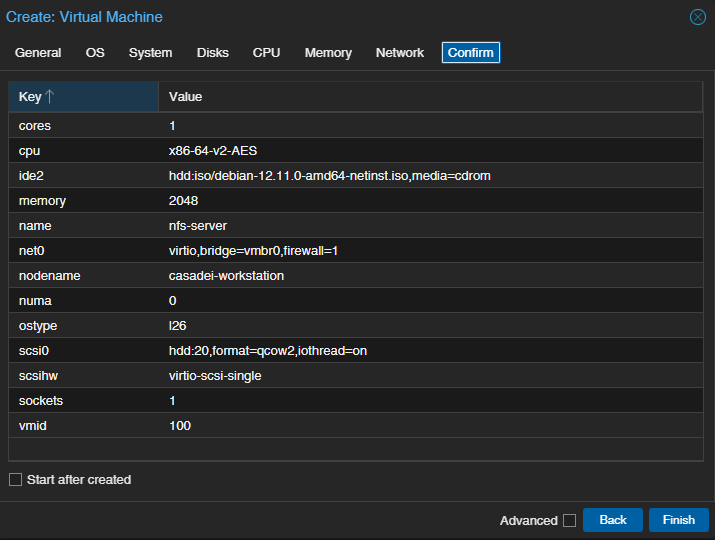
\includegraphics[scale=0.60]{images/VMNFSServer.png}
    \caption{Creazione della macchina virtuale per il server NFSv4}
\end{figure}
Si procede quindi all'installazione di Debian normale, a seguito dell'avvio della macchina
virtuale, dopodiché procedo ad installare tutti i pacchetti necessari, a partire da docker:
\subsubsection{Installazione di Docker Engine e Compose}
Dalla documentazione ufficiale di Docker, aggiungiamo la chiave \Gls{GPG}
per poter installare il pacchetto:
\begin{Verbatim}[numbers=left,breaklines]
    # Add Docker's official GPG key:
    sudo apt-get update
    sudo apt-get install ca-certificates curl
    sudo install -m 0755 -d /etc/apt/keyrings
    sudo curl -fsSL https://download.docker.com/linux/debian/gpg -o /etc/apt/keyrings/docker.asc
    sudo chmod a+r /etc/apt/keyrings/docker.asc

    # Add the repository to Apt sources:
    echo \
    "deb [arch=$(dpkg --print-architecture) signed-by=/etc/apt/keyrings/docker.asc] https://download.docker.com/linux/debian \
    $(. /etc/os-release && echo "$VERSION_CODENAME") stable" | \
    sudo tee /etc/apt/sources.list.d/docker.list > /dev/null
    sudo apt-get update
\end{Verbatim}
E installimo i pacchetti:
\begin{Verbatim}[numbers=left,breaklines]
    sudo apt-get install docker-ce docker-ce-cli containerd.io docker-buildx-plugin docker-compose-plugin
\end{Verbatim}
provando ad eseguire il comando:
\begin{Verbatim}[numbers=left]
    docker ps
\end{Verbatim}
otteniamo:
\begin{figure}[H]
    \centering
    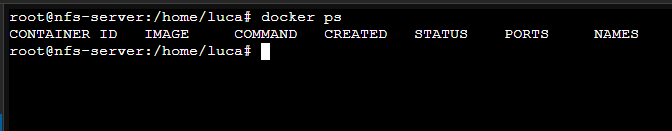
\includegraphics[scale=0.65]{images/DockerInstallato.png}
    \caption{Output di Docker PS dopo averlo installato}
\end{figure}
\subsubsection{Creazione container NFS-SERVER}
Abilitiamo i moduli NFS e NFSD dal kernel linux:
\begin{Verbatim}[numbers=left,breaklines]
    sudo modprobe {nfs,nfsd}
\end{Verbatim}
in alternativa si possono aggiungere questi due moduli nel file \textit{/etc/modules}
Come immagine per docker verrà utilizzata \href{https://hub.docker.com/r/erichough/nfs-server/}{\textbf{nfs-server}}
e verrà configurata mediante il seguente script compose:
\begin{Verbatim}[numbers=left,breaklines]
    services:
        nfs-server:
            image: erichough/nfs-server
            container_name: nfs-server
            restart: unless-stopped
            # Necessario perché il protocollo
            # usa delle direttive a livello di kernel
            privileged: true
            ports:
            - "2049:2049" # NFS (Vedi relazione)
            # - "111:111" # RPC (Queste porte sarebbero necessarie per supportare V3, non ci interessa per questo progetto)
            # - "32765:32765" # mountd
            # - "32767:32767" # statd
            environment:
            # Questo è un argument del server nfs
            # che indica la cartella dentro al container
            # da esportare con il protocollo, potrebbero
            # essercene diverse.
            - NFS_EXPORT_0=/exports
            volumes:
            # Espone la cartella interna esportata prima
            # fuori dal container con una mappatura bind
            - /srv/nfs:/exports
\end{Verbatim}
Dopo aver creato lo script ed eseguito "docker compose up" per farlo partire, nfs-server dovrebbe darci il seguente output:
\begin{figure}[H]
    \centering
    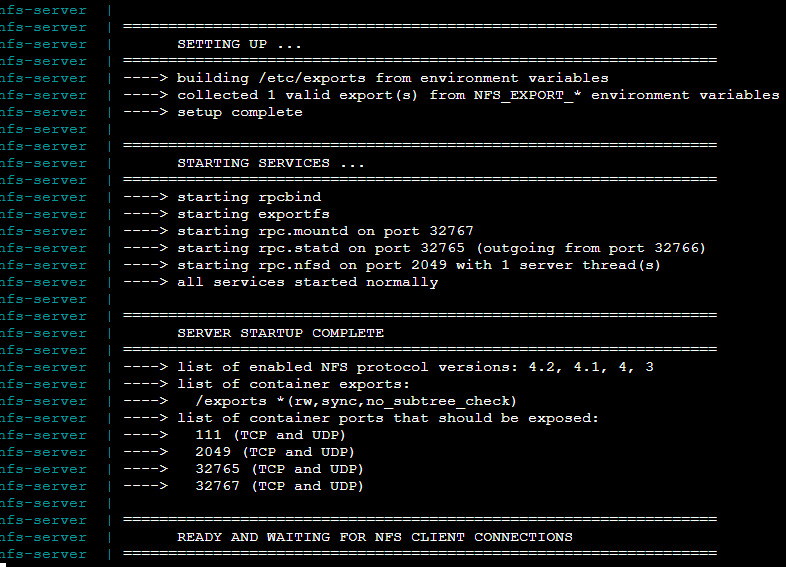
\includegraphics[scale=0.30]{images/NFSSettato.png}
    \caption{Dopo docker compose up}
\end{figure}
\printglossaries
\printbibliography
\end{document}